

Beckhoff ist ein internationales Unternehmen, welches 1980 von Hans Beckhoff gegründet wurde. Das Unternehmen realisiert offene Automatisierungssysteme. Bekannt wurde das Unternehmen vor allem in dem Bereich Industrie-PC und das zugehörige Softwaresystem Twincat. Die Produkte, welche von Industrie-PCs, Steuerungssystemen und Softwaretools reichen, werden vor allem in der Gebäude-Automatisierung und für die Steuerung von Maschinen verwendet. Konkret geht es um automatisierte Prozesse, die vor allem in der Fertigung eine große Rolle spielen. Auch die Effizienz und die Energiebilanz des Anwenders können gesteigert werden. In der Firma Flexsolution kann mit den Systemen von Beckhoff vom Licht, über Schalosien und Fertigungsmaschinen alles gesteuert werden.

Entwickelt werden solche Anwendungen in der Software Twincat mit einer von Beckhoff entwickelten Programmiersprache.
\setauthor{Marcel Pouget}


Twincat bietet den Vorteil, dass die Codeänderungen schnell und unkompliziert angepasst werden. So können, ohne dass etwas kompiliert werden muss, Anpassungen getätigt werden. Außerdem ist es möglich, direkt die Werte der Variablen zu sehen, während das Programm noch läuft. Dies erlaubt es, schnell einzugreifen und alles zu überwachen.

\begin{figure}[h t]
  \centering
  \includegraphics[scale=0.2]{pics/twincat übersicht.png}
  \caption{So sieht die Twincat Übersicht aus}
  \label{fig:impl:TwincatÜbersicht}
\end{figure}

Eine weitere Besonderheit ist die Art, wie der Code ausgeführt wird. Denn in einer Beckhoff-Steuerung wird nach einem festgelegten Zyklus der Programmcode von oben nach unten ausgeführt. Es werden dabei nur Operationen wie 'if, iflse', mathematische Operationen, Zuweisungen und timer unterstützt.

Um das Warten der Software für die Mitarbeiter*innen der Firma einfach zu gestalten, wurde nach Abschluss des Projektes die Funktion des Chargecontrollers mit der Hilfe eines Mitarbeiters für Beckhof optimiert. Dies gibt den Mitarbeitern die Möglichkeit, die Software zu erweitern, auf mögliche Bugs zu reagieren oder Änderungen durchzuführen. Durch die Anpassung für Twincat werden dem zuständigen Mitarbeiter*innen die Deployments auf dem Raspberry Pi erspart. So sieht zum Beispiel der Code für die Wallboxen aus: \ref{fig:impl:TwincatWallbox}
\cite{beckhoffWikipedia}
\cite{beckhofftwincat}
\cite{beckhoffpage}


\begin{figure}[h t]
  \centering
  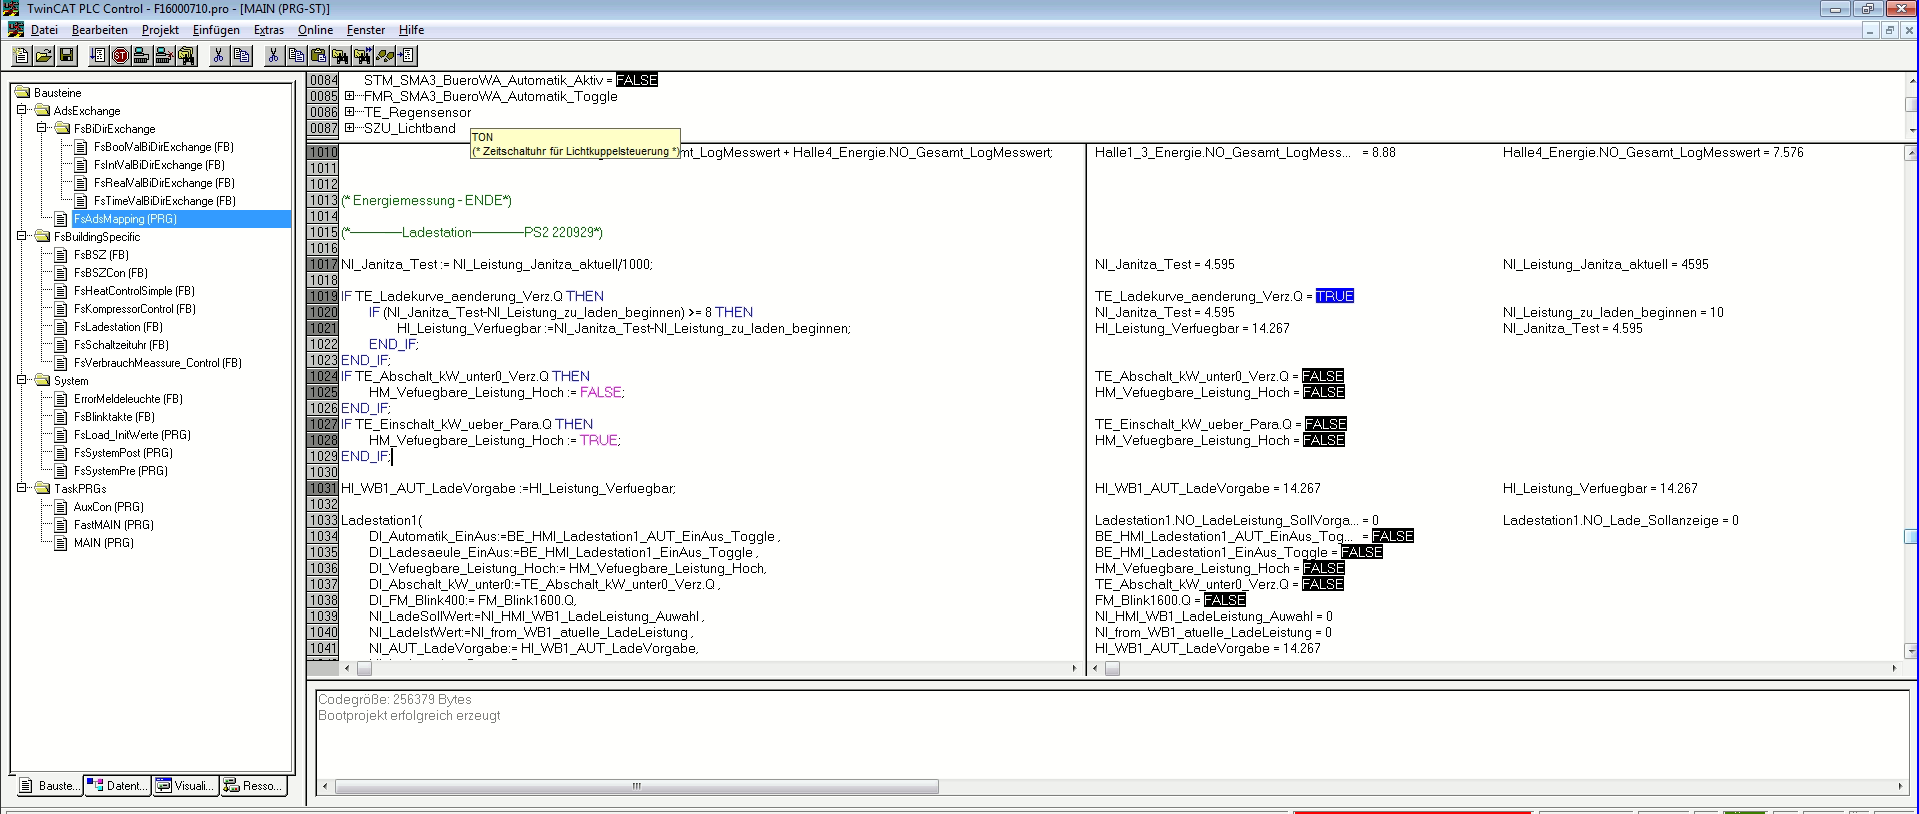
\includegraphics[scale=0.2]{pics/LadestationTwincat.png}
  \caption{Abschnitt der Wallboxen in Twincat}
  \label{fig:impl:TwincatWallbox}
\end{figure}
